На рисунке \ref{fig:PL_top} представлена схема программируемой логики.\par 
\begin{figure}[ht]
    \centering
    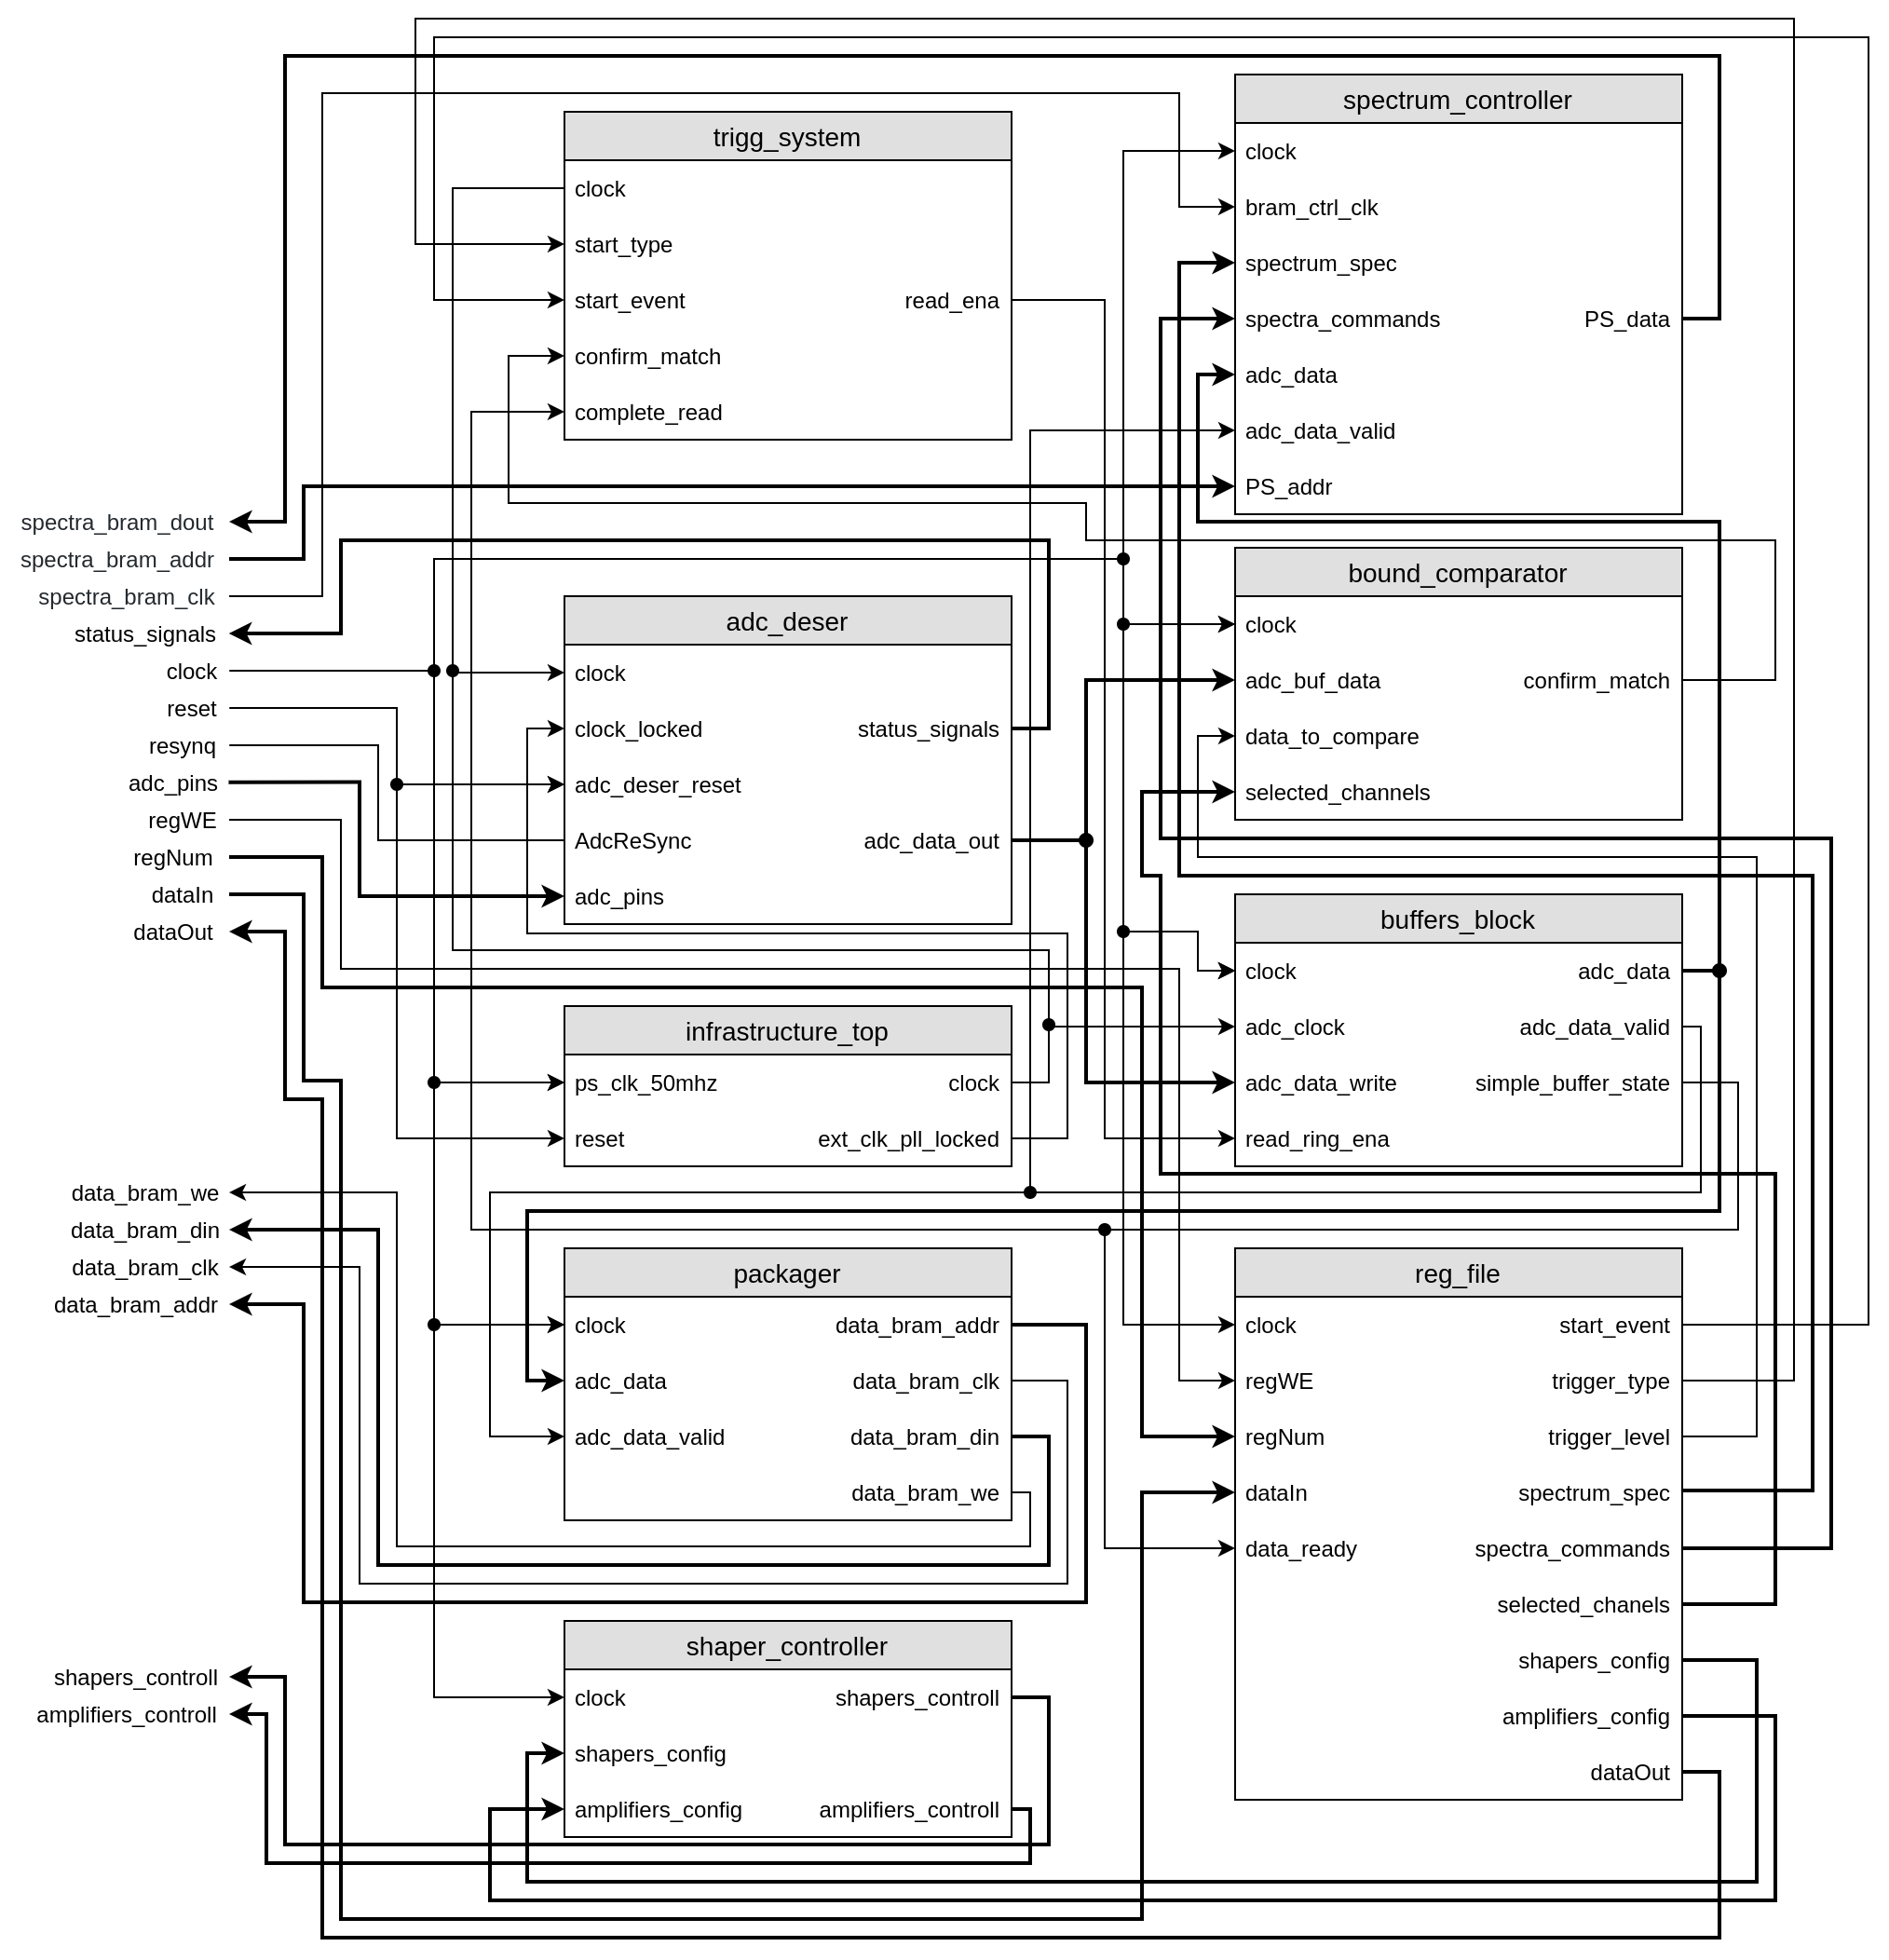
\includegraphics[width=1\linewidth]{PL_top.png}
    \caption{Блок-схема программируемой логики}
    \label{fig:PL_top}
\end{figure}
Программируемая логика состоит из 9 блоков, краткое описание который представлено в таблице 2.\par% \ref{tab:PL_top_blocks}\par
\begin{table}[ht] \label{tab:PL_top_blocks}
    \caption{Блоки программируемой логики}
   % \begin{tabular}{|>{\centering\arraybackslash}p{0.45\textwidth}|>{\centering\arraybackslash}p{0.45\textwidth}|}
    \begin{tabular}{|p{0.45\textwidth}|p{0.5\textwidth}|}
        \hline
        Наименование блока & Описание \\
        \hline
        adc\_deser & Конвертирует упакованные последовательно данные АЦП в численные значения \\
        \hline
        infrastructure\_top & Обеспечивает тактовую частоту для некоторых модулей \\
        \hline
        buffers\_block & Буферизует входные данные \\
        \hline
        trigg\_system & Генерирует сигнал для сохранения данных \\
        \hline
        bound\_comparator & Выполняет сравнение входящих данных с заданными порогами \\
        \hline
        spectra\_controller & Производит обработку данных для набора статистики \\
        \hline
        shaper\_controller & Осуществляет управление формирователями сигналов \\
        \hline
        reg\_file & Реализует блок виртуальных регистров \\
        \hline
        packager & Упаковывает данные и передаёт их в процессорную систему \\
        \hline
    \end{tabular}
\end{table}
\textbf{Десериализатор adc\_deser}\par
Одним из основных элементов стенда является АЦП AD-9253. Преобразователь работает на 100 МГц параллельно в 4-х каналах. Данные с разрешением 14 бит передаются по протоколу LVDS. Этот стандарт предполагает передачу информации в последовательно-упакованном виде по 2 каналам на каждый вход. На рисунке \ref{fig:ADC_time_diagram} представлена временная диаграмма работы АЦП.\par
\begin{figure}[ht]
    \centering
    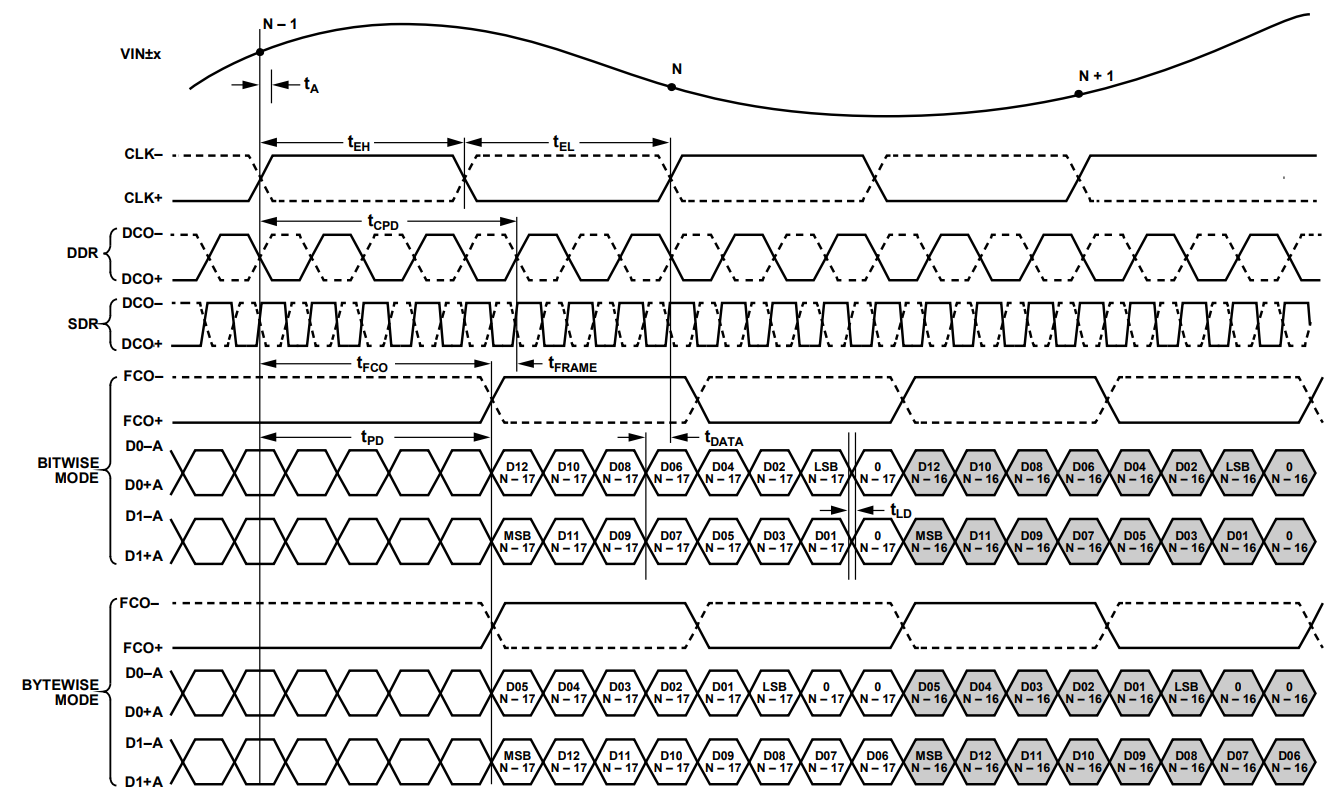
\includegraphics[width=1\linewidth]{ADC_time_diagram.png}
    \caption{Временная диаграмма работы АЦП}
    \label{fig:ADC_time_diagram}
\end{figure}
Каждый такт работы АЦП производится оцифровка входного аналогового сигнала. Как видно из временной диаграммы, полученные данные отправляются за 1 такт через 17 тактов после оцифровки по двум каналам. Представляться они могут в одном из двух вариантов: побитовый (bitewise mode) и побайтовый (bytewise mode). Данные режимы отличаются последовательностью упаковки битов --- в разных каналах передаются либо четные и нечётные биты, либо младший и старший байты соответственно. В настоящей работе выбран побитовый режим.\par
Также в работе АЦП участвуют 2 вспомогательных сигнала --- кадровый строб, отвечающий за разделение набора бит на кадры оцифровки, и тактовый сигнал передачи данных, который размечает биты внутри каждого кадра.\par
Таким образом, возникает необходимость реализации модуля, осуществляющего конвертацию последовательности бит, поступающей из АЦП, в удобное для обработки численное значение. Так как процесс упаковки бит в определённую последовательность называется сериализацией, то обратную операцию можно назвать десериализаций, а соответствующий модуль --- десериализатором. Его сигналы изображены на рисунке \ref{fig:adc_deser}.\par
\begin{figure}[ht]
    \centering
    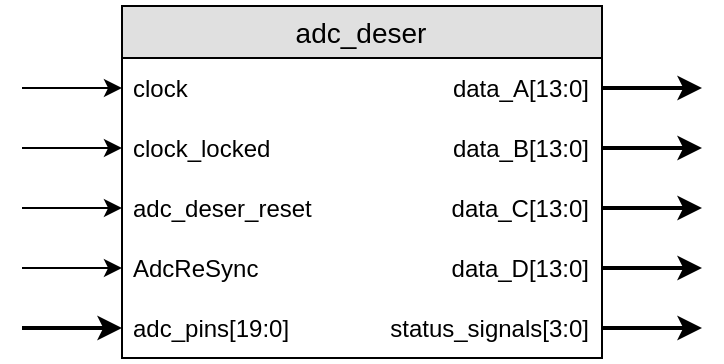
\includegraphics[width=0.5\linewidth]{adc_deser.png}
    \caption{Сигналы модуля десериализатора}
    \label{fig:adc_deser}
\end{figure}
Модуль был разработан ранее на основе готового интерфейса компании Xilinx, поэтому подробного описания его работы приведено не будет. Стоит лишь отметить, что входные данные принимаются через набор сигналов \texttt{adc\_pins}, а десериализованные значения подаются на выход через сигналы \texttt{data\_i}.\par
\textbf{Модуль infrastructure\_top}\par
Блок \texttt{infrastructure\_top} в настоящее время содержит лишь модуль фазовой автоподстройки частоты (ФАПЧ), необходимый для генерации тактового сигнала для работы АЦП и блоков, которые занимаются обработкой входных данных и их буферизацией (модули десериализатора и блока буферов). Как и десериализатор модуль ФАПЧ был разработан ранее с использованием библиотеки сложных функциональных блоков и рассматриваться подробно не будет. Сигналы модуля \texttt{infrastructure\_top}, в котором расположен ФАПЧ изображены на рисунке \ref{fig:infrastructure_top}.\par
\begin{figure}[ht]
    \centering
    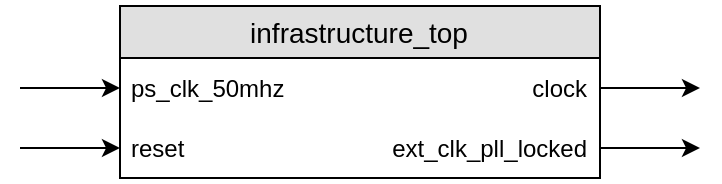
\includegraphics[width=0.5\linewidth]{infrastructure_top.png}
    \caption{Сигналы модуля infrastructure\_top}
    \label{fig:infrastructure_top}
\end{figure}
\textbf{Блок буферов buffers\_block}\par
В силу случайного характера возникновения полезных событий возникает необходимость временного хранения определённого числа последних измерений с АЦП. Для решения задачи был разработан модуль блока буферов, сигналы которого изображены на рисунке \ref{fig:buffers_block}.\par
\begin{figure}[ht]
    \centering
    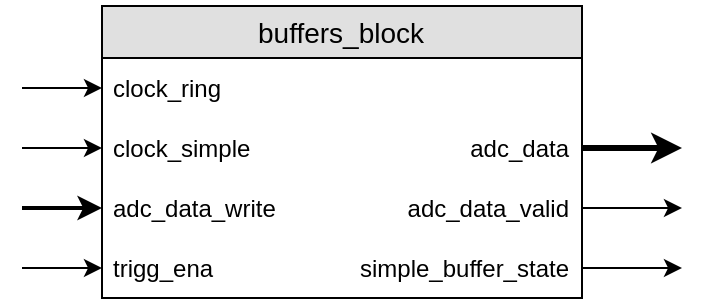
\includegraphics[width=0.5\linewidth]{buffers_block.png}
    \caption{Сигналы модуля блока буферов}
    \label{fig:buffers_block}
\end{figure}
Блок содержит в себе 2 модуля RAM памяти c раздельными портами чтения/записи данных. Первый является кольцевым буфером и непрерывно записывает данные АЦП. Это позволяет вычитывать при необходимости данные АЦП, пришедшие до сигнала триггерной системы. Такая необходимость обусловлена возможными задержками сигнала триггера, а также потребностью иметь небольшую "предысторию" осциллограммы перед достижением сигнала порогового значения.\par
Второй модуль памяти выполняет функцию простого буфера, в который временно будут выгружаться полезные данные при возникновении сигнала триггерной системы. Главной задачей такого буфера является хранение данных для гарантированного считывания и передачи их в процессорную систему.\par
Объём простого буфера определяется необходимым размером осциллограммы, который, в свою очередь, зависит от максимального времени высвечивания кристалла. В настоящей работе объём простого буфера установлен 128 кадрами. Такой размер позволяет поместить в одну осциллограмму данные, оцифрованные за промежуток времени порядка 1 мкс при работе АЦП на 100 МГц. Объём кольцевого буфера, в свою очередь, определяется максимальным количеством данных "предыстории", необходимых для анализа. Из свойств сцинтилляционных кристаллов было принято решение об использовании 64 кадров.\par
Модуль \texttt{buffers\_block} имеет два входных тактовых сигнала -- \texttt{clock\_ring} и \texttt{clock\_simple}. Система на кристалле работает на 50 МГц, следовательно, именно на этой частоте должны выгружаться данные в процессорную часть. При этом АЦП работает на 100 МГц. Здесь кроется ещё одна немаловажная задача простого буфера: переход данных из одного домена тактовой частоты в другой. Таким образом, поток данных поступает в блок на тактовом сигнале работы АЦП, а полезная информация выдаётся на частоте работы системы на кристалле.\par
Из рисунка видно, что модуль также содержит следующие входные сигналы: \texttt{adc\_data\_write} -- входные данные с АЦП, \texttt{trigg\_ena} -- сигнал триггерной системы о возникновении полезного события. Можно заметить, что выходной набор \texttt{adc\_data} содержит большее число сигналов, чем входной \texttt{adc\_data\_write}. Это связано с добавлением к данным по 2 бита, идентифицирующих их отношение к определённому каналу. Таким образом, значение каждой оцифровки хранится ровно в двух байтах.\par
\textbf{Триггерная система trigg\_system}\par
Как было сказано ранее, для сохранения данных с АЦП в буфер и последующей их передачи в процессор необходим сигнал, сообщающий о возникновении полезного события. Генерацией такого сигнала занимается модуль триггерной системы, сигналы которого изображены на рисунке~\ref{fig:trigg_system}.\par
\begin{figure}[ht]
    \centering
    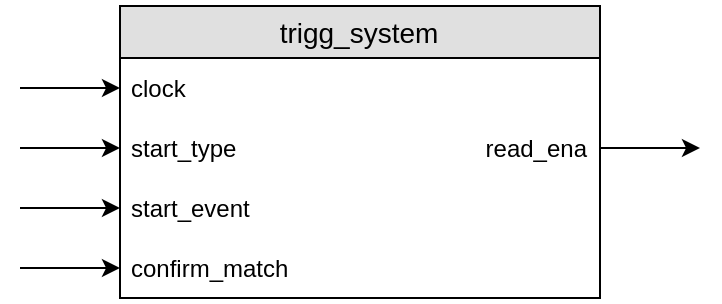
\includegraphics[width=0.5\linewidth]{trigg_system.png}
    \caption{Сигналы модуля триггерной системы}
    \label{fig:trigg_system}
\end{figure}
Триггерная система может работать в двух режимах, задаваемых сигналом \texttt{start\_type}: принудительно и по порогу. В первом случае модуль отработает сразу при появлении сигнала старта на входе \texttt{start\_event}. В режиме срабатывания по порогу триггер сгенерирует разрешение на запись только при появлении на входе \texttt{confirm\_match} высокого уровня от модуля компаратора \texttt{bound\_comparator}.\par
\textbf{Компаратор bound\_comparator}\par
Компаратор осуществляет сравнение текущих оцифрованных данных АЦП с заданными оператором значениями порогов. Это необходимо для корректного функционирования триггерной системы в соответствующем режиме работы. Сигналы блока изображены на рисунке \ref{fig:bound_comparator}.\par
\begin{figure}[ht]
    \centering
    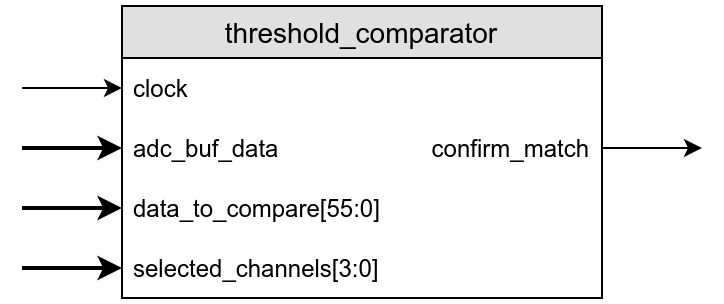
\includegraphics[width=0.5\linewidth]{bound_comparator.png}
    \caption{Сигналы модуля компаратора}
    \label{fig:bound_comparator}
\end{figure}
Данный модуль функционирует на тактовой частоте работы АЦП, т.к. он должен непрерывно сравнивать каждое оцифрованное значение, поступающее через вход \texttt{adc\_buf\_data}. При достижении или превышении порогового значения модуль формирует на выходном сигнале \texttt{confirm\_match} логическую единицу, а в противоположном случае ноль. Порог для каждого канала задаётся отдельно с помощью сигналов \texttt{data\_to\_compare}. Стоит отметить, что реализована возможность выбирать каналы, выполнение условий по которым повлечёт срабатывание модуля. Оператор может назначать их в режиме логического ИЛИ: система выдаст сигнал при срабатывании компаратора хотя бы по одному из выбранных каналов. Эта информация поступает в блок компаратора через сигналы \texttt{selected\_channels}.\par
\textbf{Модуль набора статистики spectra\_controller}\par
Для исследования сцинтилляционных кристаллов оказываются полезными не только осциллограммы высвечивания, но также статистика по определённому количеству кадров. Для набора таких данных реализован отдельный модуль, сигналы которого изображены на рисунке(\ref{fig:spectra_controller}).\par
\begin{figure}[ht]
    \centering
    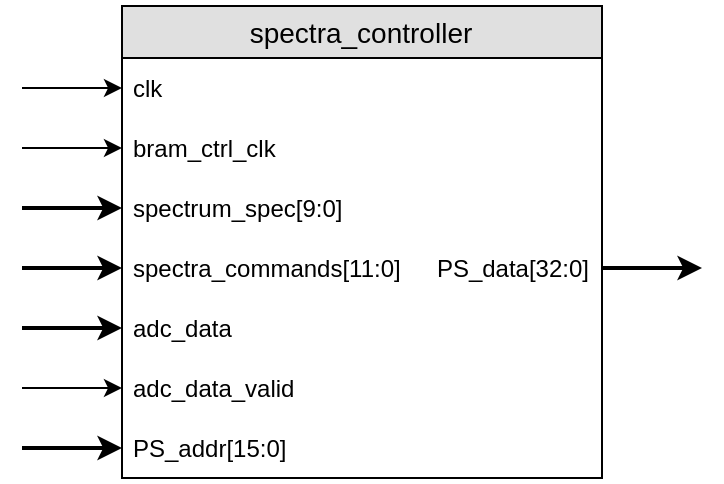
\includegraphics[width=0.5\linewidth]{spectra_controller.png}
    \caption{Сигналы модуля набора статистики}
    \label{fig:spectra_controller}
\end{figure}
Гистограммы нужны двух типов: по максимальному значению и значению определённого измерения каждого кадра. Для выполнения этих задач был разработан модуль \texttt{spectrum\_creator}, который способен находить самое большое значение переданной ему осциллограммы в определённом канале и, исходя из него, генерировать сигнал о необходимости инкрементировать соответствующий счетчик, расположенный в двухпортовой памяти. Вместо поиска максимума есть возможность задать конкретное измерение. Исходя из требований эксперимента было принято решение, что на каждый канал будет достаточно одновременного набора гистограмм по максимальному значению и по двум заданным точкам. Таким образом, на каждый канал необходимо по три вышеописанных модуля. Блок \texttt{spectra\_controller} является объединением двенадцати таких элементов и модуля \texttt{spectra\_memory}, содержащего в себе двенадцать блоков двухпортовой памяти. Чтение и запись данных со стороны программируемой логики может производиться параллельно во все блоки памяти модуля \texttt{spectra\_memory}, при этом для чтения в процессорную систему реализовано общее адресное пространство по всем блокам памяти.\par
Для работы всей системы к модулю подведён тактовый сигнал \texttt{clk}, данные с блока буферов \texttt{adc\_data} и сигнал их готовности \texttt{adc\_data\_valid}. Также для настройки собираемой статистики присутствует канал \\\texttt{spectra\_params} --- через него оператор может задавать количество корзин и выбранное измерение осциллограммы для гистограмм второго типа. Выходные данные передаются в процессорную часть с помощью сигналов \texttt{bram\_ctrl\_clk}, \texttt{PS\_addr} и \texttt{PS\_data}.\par
\textbf{Модуль управления блоком усилителей и формирователей shapers\_controller}\par
Сгенерированный сигнал фотоприёмника, попадая на стенд, усиливается и проходит через блок формирователя. На стенде предусмотрена возможность выставлять различные коэффициенты усиления и времена формирования для более точной настройки при работе с различными кристаллами.\par
Для переключения времени формирования сигнала на плате установлены электронные ключи. Управление ими реализовывается сигналами рассматриваемого модуля \texttt{shapers\_controller} (рисунок \ref{fig:shapers_controller}).\par
\begin{figure}[ht]
    \centering
    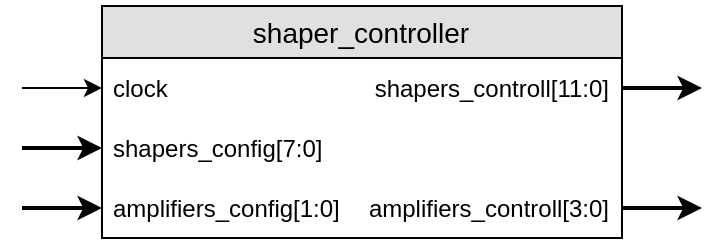
\includegraphics[width=0.5\linewidth]{shapers_controller.png}
    \caption{Сигналы модуля shapers\_controller}
    \label{fig:shapers_controller}
\end{figure}
Блок получает информацию о необходимых настройках через сигнал \texttt{shapers\_config}. Выходные сигналы \texttt{shapers\_controll} идут непосредственно к ключам.\par
Усилители, в отличие от формирователей, имеют согласованные коэффициенты усиления: 1, 2, 4 и 5. Таким образом, их состояние можно задать всего двумя битами. Их управление осуществляется в этом же блоке с соответствующими сигналами \texttt{amplifiers\_config} и \texttt{amplifiers\_controll}.\par
\textbf{Модуль виртуальных регистров reg\_file}\par
Данный модуль содержит в себе виртуальные регистры, с которыми работает блок \texttt{reg\_interface} процессорной системы. Сигналы блока изображены на рисунке \ref{fig:reg_file}. \par
\begin{figure}[ht]
    \centering
    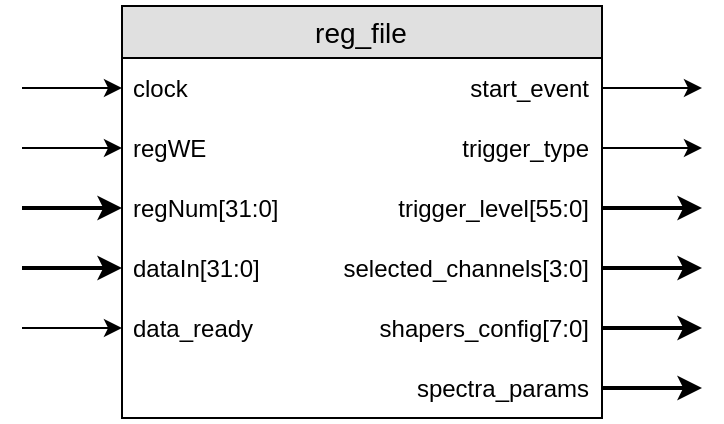
\includegraphics[width=0.5\linewidth]{reg_file.png}
    \caption{Сигналы модуля reg\_file}
    \label{fig:reg_file}
\end{figure}
При записи данных модуль получает на вход номер виртуального регистра и желаемое значение для записи. После подачи логической единицы в сигнал \texttt{regWE} входящая информация обрабатывается и, в зависимости от регистра, выставляется в определённый сигнал для соответствующего модуля.\par
Для чтения используется сигнал \texttt{dataOut}, в который передаются данные из регистра по выставленному номеру. Среди входных сигналов можно заметить сигнал \texttt{data\_ready}, передающий информацию о состоянии данных. При возникновении на нём единицы процессорная часть может получить сигнал о том, что данные готовы для считывания.\par
\textbf{Упаковщик packager}\par
Модуль упаковщика служит для отправки данных в двухпортовую память процессорной системы. Его сигналы изображены на рисунке \ref{fig:packager}.\par 
\begin{figure}[ht]
    \centering
    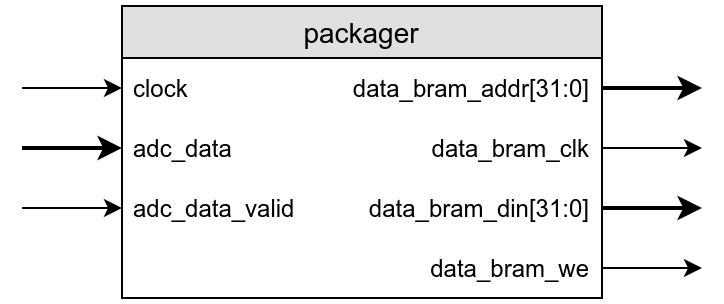
\includegraphics[width=0.5\linewidth]{packager.png}
    \caption{Сигналы модуля packager}
    \label{fig:packager}
\end{figure}
При возникновении высокого уровня на сигнале статуса данных \texttt{adc\_data\_valid} модуль отправляет информацию из сигнала \texttt{adc\_data}, выставляя адреса в \texttt{data\_bram\_addr}, данные в \texttt{data\_bram\_din} и логическую единицу в \texttt{data\_bram\_we}.\par
